\documentclass{article}
\usepackage[utf8]{inputenc}

\title{Homework 2 Report}
\author{Benny Chen}
\date{\today}

\usepackage{color}
\usepackage{amsthm}
\usepackage{amssymb} 
\usepackage{amsmath}
\usepackage{listings}
\usepackage{xcolor}
\usepackage{listings}
\usepackage{graphicx}
\usepackage[hidelinks]{hyperref}

\definecolor{codegreen}{rgb}{0,0.6,0}
\definecolor{codegray}{rgb}{0.5,0.5,0.5}
\definecolor{codepurple}{rgb}{0.58,0,0.82}
\definecolor{backcolour}{rgb}{0.95,0.95,0.92}

\lstdefinestyle{mystyle}{
    backgroundcolor=\color{backcolour},   
    commentstyle=\color{codegreen},
    keywordstyle=\color{magenta},
    numberstyle=\tiny\color{codegray},
    stringstyle=\color{codepurple},
    basicstyle=\ttfamily\footnotesize,
    breakatwhitespace=false,         
    breaklines=true,                 
    captionpos=b,                    
    keepspaces=true,                 
    numbers=left,                    
    numbersep=5pt,                  
    showspaces=false,                
    showstringspaces=false,
    showtabs=false,                  
    tabsize=2
}

\lstset{style=mystyle}

\begin{document}

\maketitle

\section{Problem 1 Test Cases}

\begin{center}
    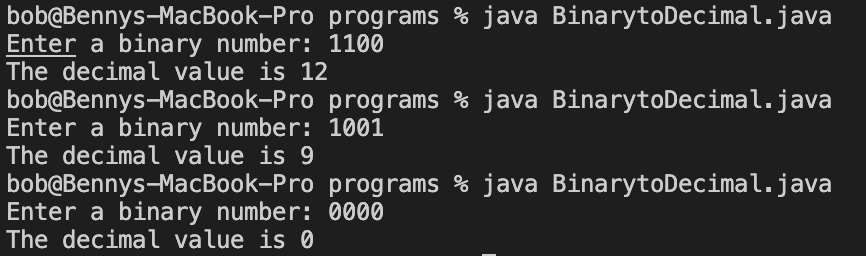
\includegraphics[width=\textwidth]{./images/binarytodecimal}
\end{center}

\section{Problem 2 Test Cases}

\begin{center}
    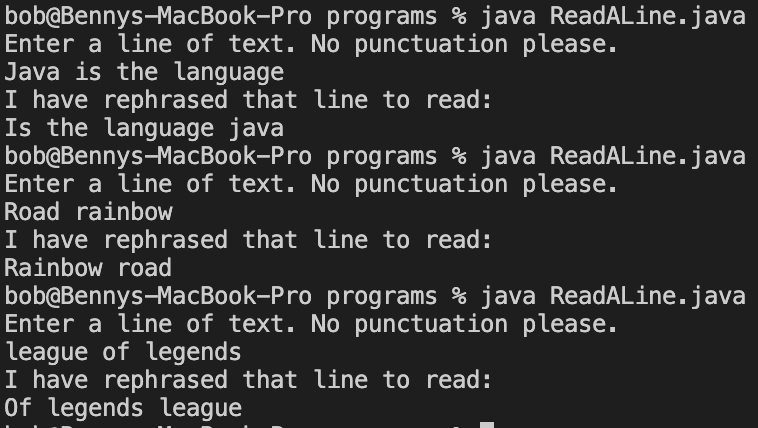
\includegraphics[width=\textwidth]{./images/readline.png}
\end{center}

\section{Problem 3 Test Cases}

\begin{center}
    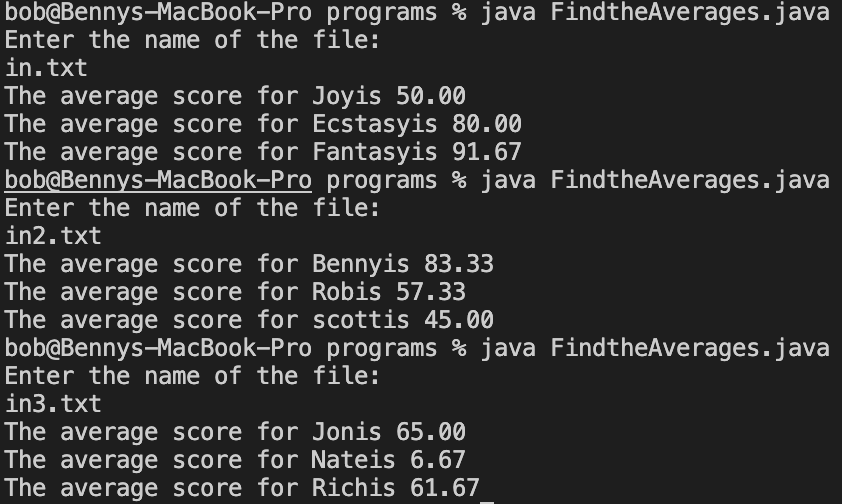
\includegraphics[width=\textwidth]{./images/findaverages.png}
\end{center}

\section{Problem 4 Test Cases}

\begin{center}
    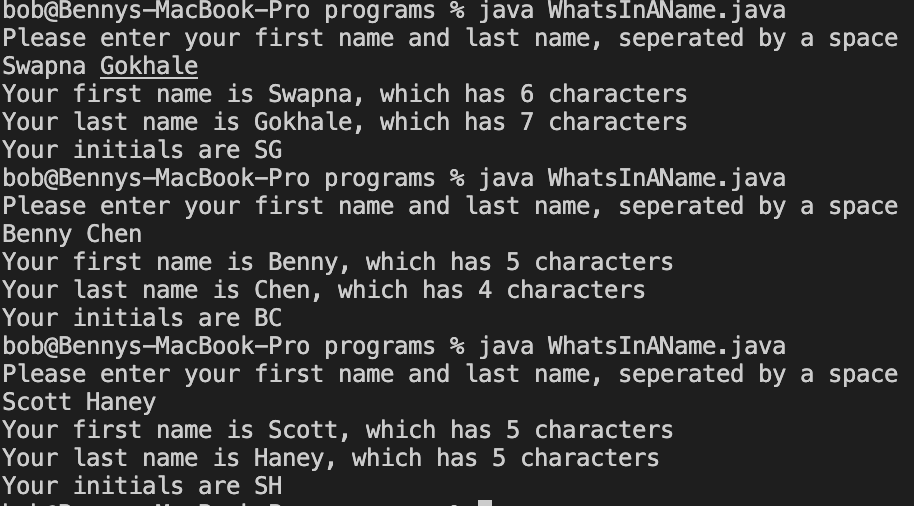
\includegraphics[width=\textwidth]{./images/name.png}
\end{center}

\end{document}

